\documentclass[12pt,letterpaper]{article}
\usepackage{geometry}
\usepackage{blindtext}
\usepackage{float}
\usepackage{graphicx}
\usepackage{amsmath}
\usepackage{nomencl}
\usepackage{amssymb}
\usepackage{enumerate}
\usepackage{gensymb}
\usepackage{fancyhdr}
\makenomenclature

\pagestyle{fancy}
\fancyhf{}

\rhead{\small {© 2022 All Rights Reserved, Aiden Rosenberg. Unauthorised reproduction of this article is prohibited.}}
\rfoot{Page \thepage}



\begin{document}

\nomenclature{\(c\)}{Speed of light in a vacuum}
\nomenclature{\(A,B,C,D,...\)}{Spatial points}
\nomenclature{\(h\)}{Planks Constant}

\title{An examination into the validity of multi-directional speed for electromagnetic particles}
\author{Aiden Rosenberg}
\date{April 16 2022 A.D}
\maketitle
\pagenumbering{roman}
\printnomenclature

\section{Introduction}
All multifarious forms of electromagnetic radiation, e.g. photonics, follow the scientific convention that light travels a defined speed of $c= 299\,792\,458\,ms^{-1}$ in a vacuum.m. This value is denoted by the letter $c$.The metre the standard unit of measurement for the scientific community defined as the displacement of a particle from point $A$ to $B$ in a a vacuum (negligible air resistance) for $\frac{1}{299 792 458}$  of a second. The speed of light represents an integral component of our visual perception of the universe and the possibility for technological development in the electronics and photonics–used for space communications.The scientific convention that defines the speed of light is a conjecture posited by Einstein; light travels at a constant speed regardless of direction, hence implying that the speed of an emitted photon from point $A$ to $B$ travels at the same speed from $B$ to $A$ after it is reflected at point $B$.However, Einstein’s conjecture is a definition not a experimentally proven phenomenon therefore it can be assumed that the speed of an emitted photon from point $A$ to $B$ travels at  $\infty(2c)$ and from the point $B$ to $A$ at the speed of $\frac{c}{2}$. Although these values lack scientific acceptance, they remain quantifiable such that the average speed for both intervals is $c$. Scientific experimentation in the field of photonics and electromagnetism is limited to only measuring the speed of light by recording the time interval it takes for a photon to travel from A to B and the back to B, hence $c=\frac{2AB}{\Delta t}$ (average speed for both directions), if this by definition is the speed of light we assume simultaneity for all real photonic vectors. Via current technology it is impossible to measure a quantitative value for the speed of light in one direction without experiencing error in the synchronisation; this is due to interactions with special relativity or the necessity to know directional variance for accurate synchronisation. It is possible that space is anisotropic hence there could result in an intrinsic preferred direction in space time correlating with a proportional ratio to a parallel directional dependent speed of light. Evaluating the validity in our current convention of the speed of light vis-à-vis synchronism and simultaneity provides a quandary that via current technology and scientific theory it is impossible to measure a quantifiable value of the speed of light thus the Einsteins convention or any equivalent anisotropic ratio could be valid.

\section{Background (Phonics \& Special relativity)}
All forms of electromagnetic radiation (EM) including radio waves, microwaves, infrared, ultraviolet, gamma, and x-rays, travel at the average multi-directional speed of c, the speed of light. Electromagnetic radiation consists of photons, high energy particles packets that do not require a medium to propagate.  the formula for the speed of light interpreted as electromagnetic radiation consists of the following equation $c=v\cdot \lambda,$ where  $\lambda$ is the  wavelength and $v$ is the frequency of the photon; the photon travels in a straight line until collision with an atom. 
\begin{center}
    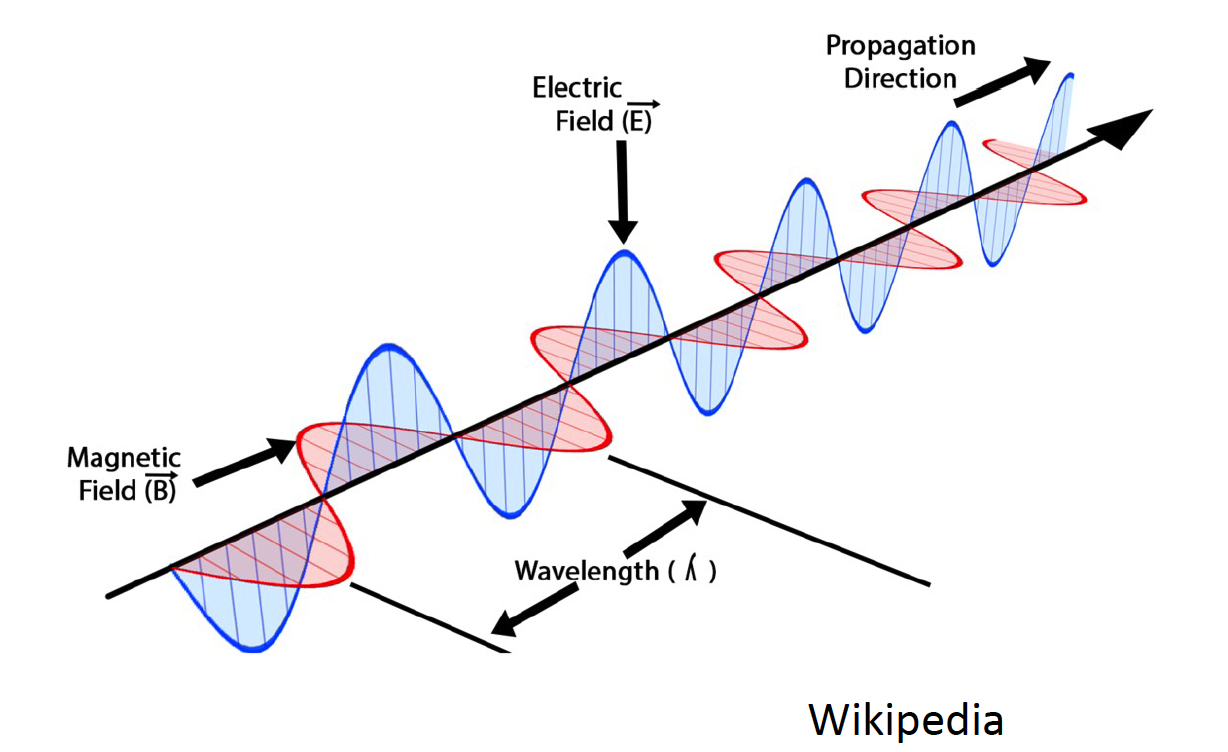
\includegraphics[width=3in]{Screenshot 2022-05-07 at 23.03.52.png}
\end{center}
In terms of photonics there is an accepted convention; “the speed of light is constant in all frames of reference; nothing in the universe travels faster than the speed of light; and objects gain relativistic mass as they are accelerated” [VI]. The speed of light constitutes the upper limit of speed for a particle; increasing the speed of the particle requires an increase in energy ergo for a particle speed to be equal to the speed of light requires infinite energy as the particle gains relativistic mass thus needing more energy to accelerate. Photons are able to travel the speed of light due to the absence of original mass therefore their mass is unable to increase with speed. The speed of a photon is also influenced by retarding forces in a medium subsequently causing resistance and energy loss in the particle. For example, electromagnetic radiation travelling through a wire (electricity) travels at approximately 90\% the speed of light, slowed due to resistance in the wire. Regardless of possible variance the round trip speed of light is a known constant $c$, this value is quantifiable and hence is a scientifically accepted constant. Our definition of speed of light is an integral component to Einstein's theory of special relativity which states that an increase in velocity of a particle the time surrounding the particle slows or dialects. In Einstein's words;
\hangindent
\begin{quote} 
If at the points $A$ and $B$ there are stationary clocks which, viewed in the stationary system, are synchronous; and if the clock at $A$ is moved with the velocity $v$ along the line $AB$ to $B$, then on its arrival at $B$ the two clocks no longer synchronise, but the clock moved from $A$ to $B$ lags behind the other which has remained at by $t'=\frac{\frac{1}{2} tv^2}{c^2}$where $t$  is the time occupied in the journey from $A$ to $B$. [I]
\end{quote} 
\begin{center}
    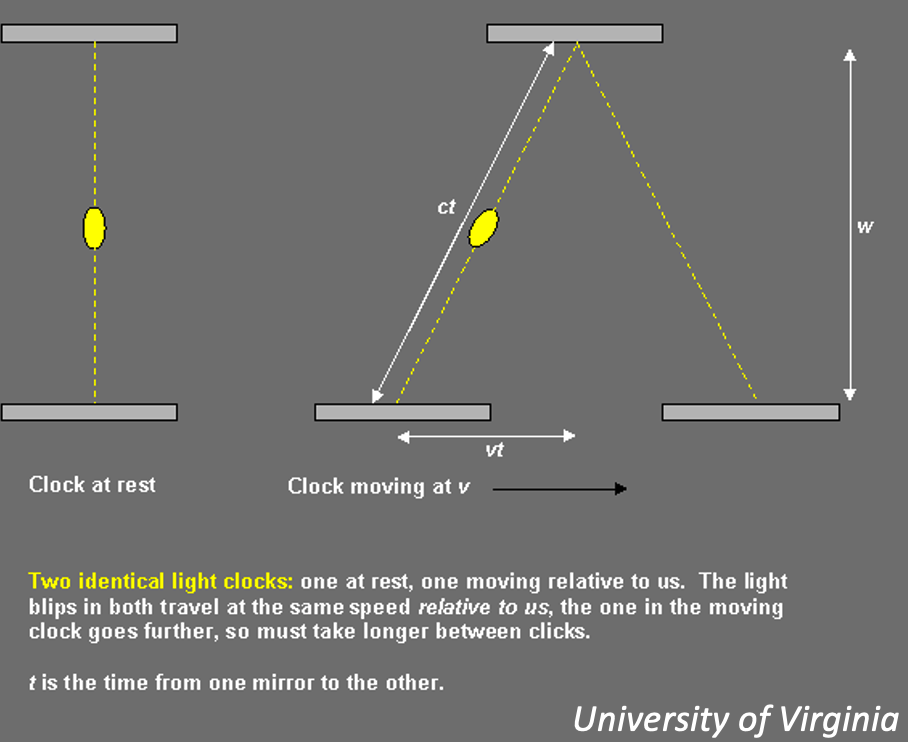
\includegraphics[width=4in]{Screenshot 2022-05-07 at 23.36.34.png}
\end{center}
The factor of special relativity is dependent on the speed of light. If we assume that the speed of light is constant in all directions it logically implies that the magnitude of relativity is the same in all directions. In Einstein's statement, the clocks are synchronised initial when they are adjacent to one another. Block B moves apart from the initial position with a velocity of $v$, due to special relativity the clocks are no longer synchronised. The nature of knowledge regarding the speed of light is circular in reasoning. If we envisage that speed is anisotropic as a variable of direction, “one [is] prevented from measuring the one-way speed of light in a given direction [since it] requires prior synchronisation of clocks and thus a prior knowledge of the speed to be measured” [VIII]. Einstein's original conjecture stated that light travels at equal speeds is “neither a supposition nor a hypothesis about the physical nature of light, but a stipulation”[I], to arrive at the conclusion of simultaneity, therefore to prove relativity we must define light by definition as unilateral in speed. It is accepted in the scientific community that all electromagnetic particles travel at unilateral speed, and thus relativity is constant in all directions. 

\section{History}
Human curiosity regarding the speed of light has remained at the forefront of scientific postulation for the past five centuries; the value of $c$ is now used as a fundamental constant in modern physics. Scientific curiosity in photonic speed was initialised by Galileo in 1638. Using two lanterns with controllable shutters, Galileo and an assistant positioned themselves upon adjacent hilltops with a known distance of separation. Galileo instructed his assistant to open his shutter at the instant he saw a beam of light. Galileo subsequently recorded the delay between the initial opening of his shutter and the time he visualised a reciprocal light from his assistant. The aforementioned photonic pulse was simulated for numerous known distances; each distance and relative time was used to approximate a value for the speed of light. Galileo was successful only in his assertion that the speed of light is approximately infinite. His experiment was limited to the technology of his time;“ the time interval between uncovering his lamp and the light is seen from the lamp of his assistant was so very small and could not be measured accurately due to the unavailability of high precision clocks during his time” [XI]. Scientific experimentation for this concept remained null until in 1728 James Bradley used stellar aberration; the angle of aberration correlates to the angular displacement for a fixed stellar body in relation to the rotation of the earth. Therefore the tangent of the angle of aberration is equal to the ratio of the velocity of the Earth $(u)$ to the velocity of light $(c)$:  $\tan \alpha = \frac{u}{c}$. In layman's terms, “he measured the apparent shift in the position of a fixed star due to rotation of earth” [XI], and “the angle that prescribes the difference between the observed position of the fixed star and the actual position at the instant of observation, known as the angle of aberration”[XII]. The time delay as a star emits light until the image is observed, is due to the finite speed of light; using the sun and the earth it was calculated that $c \approx 301000 kms^{-1}$. The basis of Einstein's theory of relativity and modern physics began with the primer efficacious and quantifiable experiment for measuring the speed of light, performed by French physicist Arnold Fizeau. “His method involved shining light from a source which was kept at a distance of about 7 km on a rotating wheel consisting of 720 teeth and rotating at about 12.6 rotations per second ”[XI], adjusting the rotational speed of the gear until the returning beam crossed the subsequent tooth.
\begin{center}
    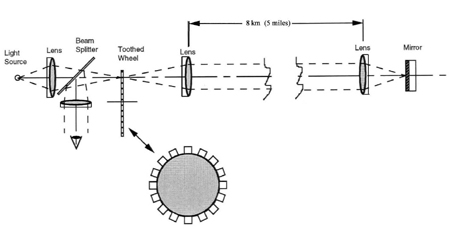
\includegraphics[]{SL gear.jpeg}\\
    \caption {Figure 1}
\end{center}

This method calculated $c \approx 313000$ms$^{-1}$ with limited sources of error only without the necessity for computerised electronic and photonic systems. Modern advancement in the field of photonic via lasers and atomic clocks follows the same quantitative modus of experimentation, finding $c = 299 792 458$ms$^{-1}$, “a definite velocity…independent of the state of motion of the emitting body” [I]. In all the aforementioned experiments, light is calculated using an average of the speed it takes light to traverse a finite distance and return to the origin of measurement (round trip average). The modern accepted value for $c$ above is the valid average speed for the light reflected off a surface until it returns to the initial position. This is proven through quantitative experimentation; the one-directional speed of light appears trivial if viewing the speed of light to be multi-directional, albeit uncertainty exists since the modus to measure light is solely an average.

\section{Einstein convention -- Time of flight}
Einstein's convention regarding synchronised clocks standardised that the speed of light is the same  defined real number for all vector positions therefore $t_B-t_A = t'_A-t'_B$   To record the speed of light requires the synchronisation of a minimum of two clocks; take two clocks $A$ and $B$ these clocks can be defined as synchronised by Einstein's convention using the laser synchronisation. For example synchronisation can occur if, “If [clock] $A$ emits a light to [clock] $B$ at time tA, let is arrive at $B$ at time tB. Similarly, let a flash emitted from $B$ at time t'B arrive at [clock] $A$ at time t'A” [III], $\therefore t_B-t_A = t'_A-t'_B$.
\begin{center}
    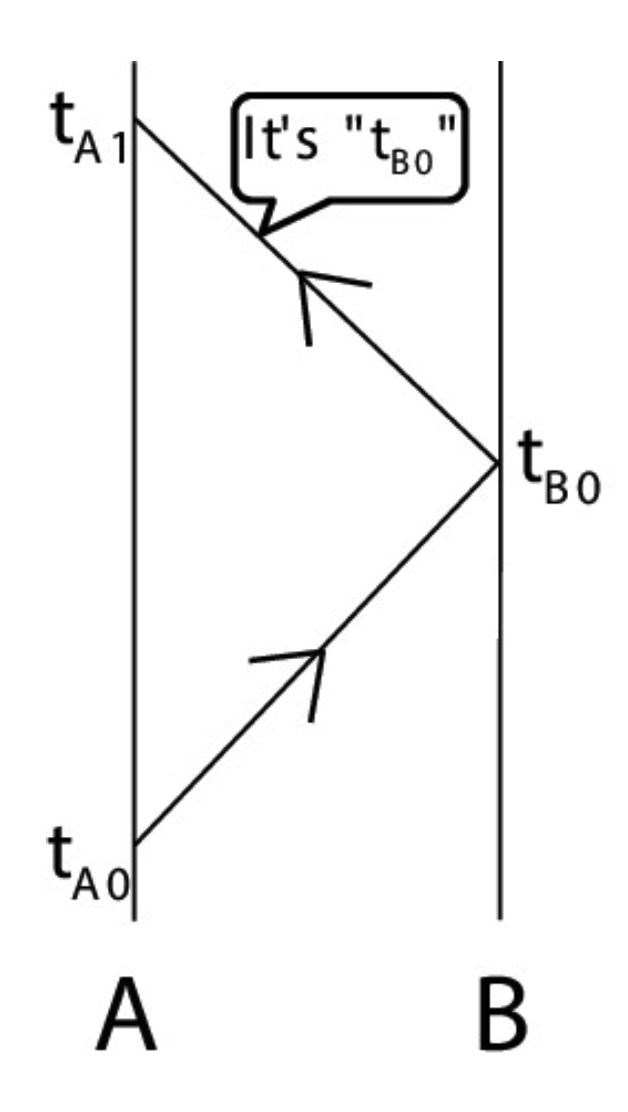
\includegraphics[width=2in]{Screenshot 2022-05-07 at 23.38.23.png}
\end{center}
Due to Einstein's convention the speed of light is the same in both directions thus clocks $A$ \& $B$ can be considered synchronised;  “by definition… the ‘time’ required by light to travel from $A$ to $B$ equals the ‘time’ it requires to travel from $B$ to $A$” according to Einstein. Once two clocks –inertial observers become synchronised any event will be recorded so that each clock observes an event simultaneously for all time determinations. For example a particle travelling from $A$ to $B$, and if both clocks' initial times are synchronous, the time recorded by clock $A$ when the particle is at point $A$ reads the same as  clock $B$ at that moment. Due to special relativity a pair of clocks will only deviate if their stationary positions of inertial observers are changed. When both clocks are synchronous “we assume the quantity $c=\frac{2AB}{t'_A-t_A} = \frac{A}{t_B-t_A}=\frac{B}{t'_A-t_B}$, to be a universal constant—the velocity of light in empty space” [I]. Assuming the speed of light is a constant and the distance between points A, & B, the time interval $A$ to $B$ is equal to the time interval from $B$ to $A$ hence we assume $c=c'$. Not only does Einstein's time convention apply to linear photonic paths but also to equilateral triangular paths and polygonal paths. 
\begin{center}
    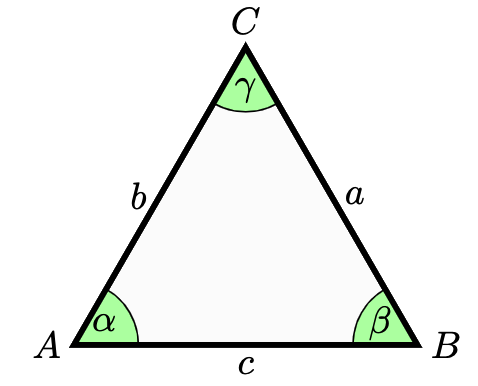
\includegraphics[width=2in]{Screenshot 2022-04-24 at 20.14.18.png}
\end{center}
For example take triangle ∆ABC on a closed path of reflections over suitable mirrors; id at each station point there exist at a clock synchronised with each respective clock on the triangle logically implies  $c=\frac {AB+BC+CA} {(t_B-t_A)+(t_C-t_B)+(t_A'-t_C)}=\frac {A}{t_B-t_A}$  if each side is of equal length. Note for polygons the vector sum of the speed of light for each side length is equal to zero ergo the particle displacement in each direction is zero. Professor Minguzzi gives a final example of Einstein's conjecture;
\begin{quote}
Consider a point $O$ and a clock at rest at 0. We define a time $t(e)$ of a generic event $e$. Emit a light beam from $O$ to $e$, where it is reflected back to $O$. Let the departure and arrival times of the light beam be $t^i(e)$ and $t^f(e)$ according to the clock at O. Define $$t(e) = \frac{t^f(e) + t^i(e)}{2}$$ This procedure assigns a time $t(e)$ to every event $e$ \…  if e is at point E, then $t^f(e)-t^i(e) =2\Bar{OE}/c $.  The one way speed of light with respect to $t$ is $c$; [maintaining this conjecture] $t(b) − t'(b) = t(a) − t'(a)$. [III]
\end{quote}
Professor Minguzzi demonstrates that synchronising two clocks at each time interval regardless of the direction for $A$ to $B$ results in an equivalent net change in time. If the time intervals are equal regardless of direction $\text {velocity}=\frac {\text{light path }} {\text { time interval}}$ In the experiment point $O$ and $E$ consist of a stationary system–physical particles do not undergo change, therefore all particles experience a determined velocity c. Einsteins convention while critical to the moderne definition of the speed of light is solely an accepted praxis for determining a universal value for the speed of light regardless of directions; while his convention is accepted it is not proven therefore $t(b)-t'(b) = t(a)-t'(a)$ only because of the assumption that the particle travels at the same speed in all directions without consideration for   Anisotropic space time.

\section{Special Relativity in Anisotropic Space}
The proof for a varying one-directional speed of light is rooted in the possibility of anisotropic space, a theory where the natural universe has a preferred direction in space-time ergo the speed of light would correspond to the anisotropic space gradient. Anisotropic theory is a rebuttal to Einstein's time of flight convention to measure the speed of light since it assumes that for the speed of light to remain constant in all directions then the nature of space time must remain isotropic- uniform regardless of vector movement.
\begin{center}
    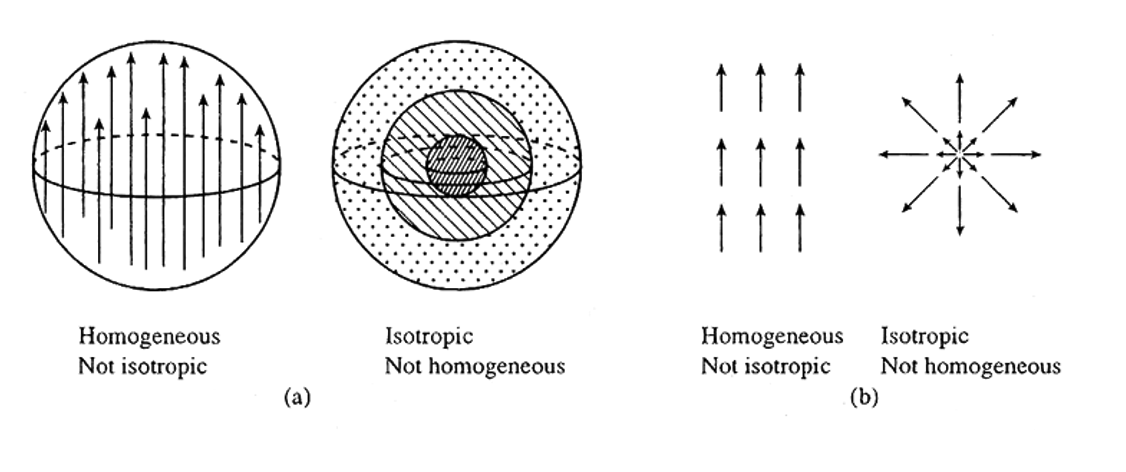
\includegraphics[width=3in]{Screenshot 2022-05-07 at 23.34.11.png}
\end{center}
“The validity of the various SR (special relativity) effects does not imply that the speed of light must be isotropic… [rather it] implicit in the SR formalism itself, foliation of the 4-dimensional spacetime into a 3-space and a 1-space” (Cahill). If the speed of light experiences directional variance than special relativity magnitude is dependent on this variance. Using a singular dimensional foliation, special relativity shows that the transversal speed of a particle time dilation is inversely proportional to its velocity; given anisotropic theory the magnitude of time dilation is directly dependent on the individual vector quantity for the relative vector of light. “Different locations in the universe could be expected to experience different levels or directions of anisotropy” [IV]. For example the most plausible theory for the prevalence of anisotropy suggests  that light travels faster in the direction parallel to the expansion of  4-dimensional spacetime, hence the movement of a photonic particle could travel a speed of  $\frac{c}{2}$  from point $A$ to $B$ and  $\infty$  from $B$ to A. To prove the conjunction between anisotropic space on the one-way velocity of light is dictated by the following equation:
$$\vec {c}\vec{(n)}=\frac{\vec n}{1+\vec \epsilon \vec n}$$ [XIV] 
 The notation $\vec {c}\vec{(n)}$ denotes the one-way velocity of light where $n$ is the vector of travel for the EM photon and $\vec \epsilon$ is the synchronisation coefficient of each corresponding clock; in Einstein convention  $\vec \epsilon=0$.  The equation above shows that the one-way velocity of light requires synchronisation dependency, if and only if the value of the synchronisation coefficient remains constant as recorded by two stationary observers. Regardless of the anisotropic relativity, both clocks remain synchronisation dependent, “making all synchronizations equivalent as long as kinematic effects for light or subliminal signals are considered” [XIV]. For example assuming the speed of light is anisotropic in clock experiments we are no longer able to assume relativistic symmetry of the time intervals hence to achieve simulating a clock on earth must compensate by dilating–displaying extra time to guide the anisotropy of the speed of light. In Rosenberg 9 † Spatial points are denoted with letters A, B, C . . . layman's terms, measuring the round trip speed of light following Einstein's convention posits that if the average speed of light between must remain constant, ergo: $$\frac {c_{AB}+c_{BA}}{t'_A-t_A}=c$$ The one directional speed of light is greater than the speed of the reciprocal direction; both speeds must average to the round-trip speed of light as discussed in the aforementioned experiments. Current experiments albeit not yet peer-reviewed “demonstrate [that] the anisotropy of the speed of light… is quite large, namely $300,000 \pm$ 400 km/s, depending on the direction of measurement relative to the Milky Way” (Cahill). The given value of anisotropy is the ratio of deviation where the relative local minima and maximum average to the round-trip speed of light; it is erroneous to visualise the discrepancy in speed using kinematics rather if we attempt synchronisation using light pulses or electricity the time deviation will correspond to anisotropy. The current value of deviation for anisotropy is a purely theoretical postulate that lacks theoretical grounding –the inclusion of this value demonstrates the finite result for the anisotropy of space time. Anisotropy is currently the only theoretical grounding to prove that the unidirectional nature of light, rather than the accepted postulate, along with Einstein's time of flight, remains conjecture due to the lack of experiment and valid theoretical grounding.

\section{Heisenberg’s Uncertainty Principle}
Proof regarding the invariance in the speed of light can also be examined via Hisenberg's
uncertainty principle (HUP); $\Delta x \cdot \Delta p =\frac{h}{4\pi}$ ($h$ represents Planck's constant), via examining individual uncertainty in the moment and position of the photon as it relates to the aforementioned modus of recording a round trip average. In Heisenberg words “Je genauer der Ort bestimmt ist, desto ungenauer ist der Impuls bekannt und umgekehrt,” which translates to “The more precisely the location is determined, the more imprecisely the momentum is known and vice versa”. It is known that the momentum of a photon is $p=\frac{h}{\lamba}$which can be used to derive the following equation $p=\frac{hf}{c}$. Therefore assuming possible uncertainties due to the photon's momentum; assuming Planck's constant and standard frequency of an emitted photon, it Rosenberg 12 can be concluded that the change (uncertainty) in momentum is inversely proportional to variance in the speed of light. Hisenberg principle is rooted in his initial postulate regarding measuring the speed of an electron using photon scanning; in a vacuum the speed of light is proportional to the speed of an electron through a medium with no resistance. 
\begin{quote}
    At the instant of time when the position is determined, that is, at the instant when the photon is scattered by the electron, the electron undergoes a discontinuous change in momentum. This change is the greater the smaller the wavelength of the light employed, i.e., the more exact the determination of the position. At the instant at which the position of the electron is known, its momentum therefore can be known only up to magnitudes which correspond to that discontinuous change; thus, the more precisely the position is determined, the less precisely the momentum is known. [XII]
\end{quote}
In layman's terms the process of measuring a photon to calculate the speed of light is indeterminable if the final position of the photon is known; the ratio between the certainty of both the position and momentum (velocity vector) is proportional to a finite constant of proximity of approximately $6.62607015 \cdot 10^{-34}$ kg$\cdot$m$^2$/s . According to “HUP…the world of the very small is inherently elusive, in this sense, the uncertainty principle assumes an epistemological (theoretical) value [limiting our quantifiable definition for] quantum particles” [X]. HUP provides a quantum framework for stating that experimenting with measuring a photon's velocity using a system of mirrors to reflect the particle is result in entropic uncertainty hence variance in the directional speed of light cannot be quantifiable determined via HDP only it assists in approximating a theoretical limit. This conjecture using HUP as a rebuttal of Einstein's initial postulates is discussed in an article published by Michael Cordin.He explains, “[Applying HUP] the emission time of the photon is uncertain over a period of time, and consequently, the photon is delocalized”; removed from a linear path. If the path of the photon is delocalized then linear regression cannot be used to calculate the speed of light since $c=\frac{2AB}{t’_{A}-t)A}$; assumes the behaviour of the particle is certain ergo travelling in linear– one-dimensional motion from $A$ to $B$; this aforementioned method uses the known displacement of the particle to calculate the velocity. For example, it can be postulated that delocalization is affected by variance in the speed of light, variance in the packets–photons intrinsic energy given by the diode, or allotropic pockets causing uncertainty in the observed photonic behaviour. He further explains that “the extent of delocalization determines the uncertainty with respect to the momentum along the flight direction, which corresponds to the total momentum of the photon, [ergo] delocalization (along the flight direction) determines the size of the momentum interval”[VII]. Delocalized photons disperse energy in uniform patterns as they move from point $A$ to $B$; in non-delocalized particles, the energy consists of small localised packers internal with the movement of the electrons. The amount of delocalisation caused by the reflection on the mirror correlates to an uncertain velocity of the photon as it progresses from $A$ to $B$, since the total energy of the photon is no longer proportional to momentum. The invariance of the velocity of a particle can be interpreted by the following equation: $\Delta x’=(c+v) \cdot \Delta t$; the large the delocalization of the particle is represented as $v$ the greater area of delocalization. In the aforementioned equation, delocalisation corresponds to the variance in the speed of light, the greater the variance implies increases the certainty of position hence decreasing the uncertainty in the position of the particle. If there is variance in the speed of light HUP remains true, since the momentum of the particle's uncertainty must be inversely proportional to the variance in $c$; assuming a known position correlates to a decreased certainty in momentum ergo variance in the speed of light.

\section{Clock Simulations \& Errors}
Examining the restrictions and conjectures provided by both Anisotropy and special relativity upon our initial postulate, allows the visualisation of the erroneous nature of the types of current analysis to measure the one way velocity of light. Postulating experiments to measure the one way speed of light must follow the following criteria; as stated by einstein: “The laws by which the states of physical systems undergo change are not affected…uniform translatory motion; [and]  any ray of light [must] move [within a set of] “stationary” coordinates [I]. With theses criteria, differentiating between the validity in results and anisotropy and special relativity allows us to reexamine errors within our initial course of inquiry targeting accurate synchronisation. For example take two clocks one at point $A$ and one respectively at point $B$; a signal of synchronisation is set form point $c$ so that $\overline {CB}= \overline {AC}$. Both segments are connected using an electric conduit; this signal consists of an electric charge sent through both wires at the same time– this experiment is congruent with an identical procedure involving light as the synchronisation calibrator. Theoretically following Einsteins synchronisation convention both clocks $A$ & $B$ will become synchronised at the instant the electrical signal (or light) is received; this conjecture is valid on the condition that, “we establish by definition that the “time” required by light to travel from $A$ to $B$ equals the “time” it requires to travel from $B$ to $A$” [I]. If the the speed of light from $\overline {CB} \neq \overline {AC}$ , and assuming $v_{CA}>v_{CB}$ it can be concluded that clock $B$ will delayed such that when measuring the speed of light the recorded value will result in a constant c, despite assuming that the speed of light is non uniform in all directions. If the speed of light is not uniform and therefore the clocks are not synchronous; first the amount to delay is infinitesimal–albeit not insignificant to scientific procedure, second the delay the accounts for the the exact the amount of time so that the speed of light will remain the same experimentally recorded value. This is due to the principle that if a delay is present the direction of the photon must move either at a faster rate to account for an equilibrium in average time, the reciprocal applies if the clock is faster hence the speed of light is slow in the corresponding vector direction. Methods of synchronisation using a translational point from the system will always result in the same aforementioned experimental uncertainty regardless of the use of GPS, light, or electric synchronisation. The second postulate regarding a methodology to affirm experimental accuracy is using special relativity as calibration. Take clocks $A$ and $B$ both positioned adjacent to one another both of these clocks can become synchronised internally so that synchronisation remains constant; now move these two clocks away from each other at the same magnitude of velocity following traditional linear regression– continue moving both clocks an equal distance and stop. It can be assumed that since both clocks moved, the magnitude of their time dilation will be equal in magnitude due to Einstein's theory of relativity. This statement is fallacious since if the speed of light is not uniform then the magnitude of special relativity will correspond to the theoretical relative vector speed of EM particles; Einstein's time convention defies his theory of relativity via the assumption that remains moot, directionality of the speed of light. The final type of experiment procedure posited is once that uses a single clock; using a piece of fibre optic cable whose path forms a perfect circle of radius $r$ light is emitted through the cable and the total time it takes for one revolution is recorded. Using the circumference of the circle $c=\frac{2\pi r}{\Delta t}$; this method is fallacious since it only calculates the average speed; as light travels in a circular path the tangent vector of travel is changing instantaneously hence velocity is recorded as an average for all vector positions. Regardless of experimental accuracy each experiment refreshes the current inability and scientific deadlock with the speed of light relative to the derivation of travel; the rebuttal aforementioned to the previous experiments form the basis of current quandary.

\section{The Greaves, Rodriguez, and Ruiz-Camacho experiment}
In 2009 physicist E. D. Greaves, A. M. Rodriguez, and J. Ruiz-Camacho performed a ‘one way speed of light experiment’ which was subsequently published in the American Journal of physics– all three physicists are instructors at Simon Bolivar University (10.4084° N, 66.8756° W).  They describe their experiment as the following;  
\begin{quote}
An instrument transmits a light beam of visible wavelength from a … modulable laser… to which is applied a modulation signal of approximately 1 MHz. The beam is amplitude-modulated. In a geodimeter without the variation the light beam is directed onto a mirror at a distant point from which it is reflected back to the instrument. The incoming light is received by a photosensor and converted to an electrical signal, and the difference in phase between the reference transmitted and the received signals is measured in a digital oscilloscope…. The timing of the light path is done by a measurement of the phase difference between the transmitted modulated signal in the instrument and the signal received by the light sensor. [II]
\end{quote}
In summary this experiment is an analysis into the differential behaviour of the reflected light waves to analyse discrepancies between the frequency and amplitude of the received signal to the transmitted signal. Vis-à-vis analysis into the photonic discrepancy increasing the distance of the reflection point linear regression was used to calculate $c=\frac{dt}{dx}$ (derivative of time with respect to position). 

\begin{figure}[H]
    \centering
    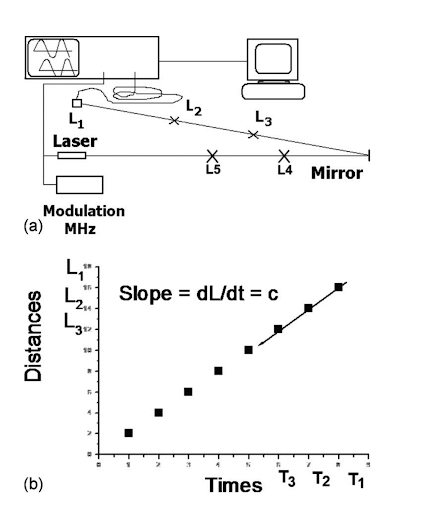
\includegraphics[width=4in]{LatinLight.png}
    \caption{Fig. 1. a Schematic diagram of the experiment to determine the one-way speed of light. b Sketch of the expected results if the one-way speed of light measurement is possible.[II]}
\end{figure}
 Within a margin of error of  2.4\% and 2.8\%  $c$ the speed of light in the direction measured was calculated as $c=3.09 \cdot 10^8 m/s$, which differs from the accepted value by 0.4\% [II]. The result of Greaves, Rodriguez, and Ruiz-Camacho experiment attempted to provide a simplistic and unifore type of experimentation to calculate the directional speed of light. Albeit their experiments were crude and simplistic once compared to the traditional experimental and quantitative research– the phase shift measured by the photonic receiver provided a finite result which corresponds to theatrical predictions. 

\section{Rebuttal to the one way speed of light experiment}
Physicist J Finkelstein–San José State University, published a one page rebuttal to Greaves, Rodriguez, and Ruiz-Camacho experiment proving that they measured the rebound trip speed of light rather than the proposed one directional speed of light. In his rebuttal his first states, “the first leg of this round trip is the light propagating from the laser to the photosensor, and the second leg is the signal going through the coaxial cable from the photosensor back to the vicinity of the laser” [V], hence the experiments hypothesis is invalidated due to the erroneous neglect for EM vector change. The experiment assumes that the resistance and time for an electrical signal corresponding to a negligible time accounted for using the round trip speed of light.  As the oscilloscope analogue channels read the imputed wavelength discrepancies the recorded data fails to account for the fixed time delay of the “fixed time delay of 79 ns… for the 23.73 m … [length of the] transmission cable”[V]. In conjunction with a resistance of the electrical signals in the data cable, the recorded speed of light is converted into electrical signals in which substance changes vector positions hence providing an unexpected unknown quantity into the initial experiment. The final error Finkelstein discusses is the death of an apparent synchronisation convention differential from Einstein's initial postulate, In the text, he states, “The authors point out that all timing is performed in a single place (the vicinity of the laser) so no convention for the synchronisation of distant clocks seems to be necessary, the assertion of a known time delay through the cable is only meaningful if one imagines having synchronised clocks at the two ends of the cable” [V]. Synchronisation is necessary to account for the delay in the second leg of the experiments so that the cable delay can be considered null in overall results. The experiment must define the synchronisation between the first leg and the clock so that the element only measures the photonic shift change in the reflected light rather than the coaxial cable. The experiment assumes an implicit and yet distant synchronisation of the photonic patterns observed; to append this issue the EM reviver could become integrated within the isolation so that the delay can be considered null. This rebuttal contributes to the necessity for continuous postulation regarding experiment theory to prove whether the speed of light is unilateral or direction-dependent; the statement remains true that the one directional speed of light is unable to be measured. 


\section{Relevance in space travel}
The question can be posited “What is the relevance of assuming variance in the speed of light, does it affect the planetary activity or will this concept remain theoretically postulated”? Determining the validity of Einstein's synchronization constant will become an integral part of interplanetary communications, in the next century. In the subsequent example, let us assume the following criterion of communication: there is an astronaut on Mars, the round trip communication delay for Mars as approximately 20 minutes, and the use of NASA Space Communications and Navigation (SCaN) network (infrared signal modulation). Scenario one is as follows
\begin{enumerate}
\item At 12:00 Huston sends a time stamped synchronisation message to Mars
\item The astronaut receives the message and assumes the time delay is 10 minutes hence
setting his clock to read 12:10. He subsequently sends a return message.
\item Huston reads the return message at the 12:20
\item Both clocks are accepted as synchronised
\end{enumerate}
Both clocks are considered synchronised assuming Einstein's convention; if the round trip delay between earth and mares is 20 minutes, hence that the one-way delay can be assumed to be 10 minutes. This scenario highlights the conjunction that the speed of light is constant regardless of direction; assuming this convention we use the known round trip delay to average each leg. Scenario one is valid if Einstein's syncretization constant is true. Now in scenario two let us assume the speed of light is not constant; scenario two is as follows:
\begin{enumerate}
\item At 12:00 Huston sends a time stamped synchronisation message to Mars
\item The astronaut receives the message and assumes the time delay is 10 minutes hence
setting his clock to read 12:10. He subsequently sends a return message.
\item Huston reads the return message at the 12:20
\item Both clocks are accepted as synchronised
\end{enumerate}
In scenario two the time delay from Earth to Mars is 20 minutes hence the astronaut clock is 10 minutes slower than the actual time on planet Earth; accounting for a constant average round trip the message is instantaneous, received at 12:20. While both NASA and Mars believe synchronisation is apparent, this error cannot be visualised after synchronisation ergo the clocks remain unsynchronised. This error in synchronisation results from knowing only the round trip time delay of the message to be sent and verified from the martian planets; similarly to the speed of light the average is known but not the directional dependent delay. In order to account for possible directional variance in the time it takes the message to be received the directional delay must be known; to synchronise two clocks to measure the speed of light (or martian delay) the variance of light (or martian delay) must be known to adjust the bounds of synchronisation so that the one directional speed (or martian delay) can be measured. In both scenarios above the time interval is the same and the average value for the delay (speed of light) is constant. It is important to note that there is an infinite number of synchronisation conjectures that can be applied. The summation of the times for both legs must be equal to the total time. In scenario 2 the time from Mars to Earth is $ \vec{c}= \infty (2c ≈ ∞)$ and from the point Earth to Mars at the speed of $\vec{c}= \frac{c}{2}$ ; averaging these speeds results in an average of � for the entire interval. As humans become an interplanetary race clock synchronisation and complete certainty regarding the speed of light will be necessary to lay the bedrock of interplanetary humanity. 
\section{Conclusion}
In the present, our inability to measure the speed of light remains an impetus for scientific postulates; it remains unknown if the light is direction-dependent or if Einstein's convention is valid; anisotropic theory, special relativity and Heisenberg's uncertainty principle all posit quantifiable uncertainty in EM speed, understanding synchronism and simultaneity may prove integral for humanity's interstellar leap. Astrophysicists commonly state that locking up at the stars is looking back in time. This statement could be fallacious since if $\vec{c}=\infty$ for a star to human vision then we are looking at the present billions of kilometres away. In conclusion, the velocity of the light remains a problem for our brightest minds to answer. 

\section{References}
\begin{enumerate}[I.]
\item A. Einstein, “Zur elektrodynamik bewegter Körper [ADP 17, 891 (1905)],” Annalen der Physik, vol. 14, no. S1, pp. 194–224, 2005. 

\item E. D. Greaves, A. M. Rodríguez, and J. Ruiz-Camacho, “A one-way speed of Light experiment,” American Journal of Physics, vol. 77, no. 10, pp. 894–896, 2009. 
\item E. Minguzzi and A. Macdonald, “Universal one-way light speed from a universal light speed over closed paths,” Foundations of Physics Letters, vol. 16, no. 6, pp. 593–604, 2003. 
\item H. Ganjitabar, “Anisotropic Special Relativity,” Jan. 2021. 
\item Finkelstein, “One-way speed of light?,” 2009. 
\item W. Davies, “Measuring the one-way speed of light,” Applied Physics Research, vol. 10, no. 6, p. 45, 2018. 
\item M. Cordin, “A justification of the invariance of the speed of light by quantum theoretical considerations,” Scientific Reports, vol. 11, no. 1, 2021. 
\item R. Anderson, I. Vetharaniam, and G. E. Stedman, “Conventionality of synchronisation, gauge dependence and test theories of relativity,” Physics Reports, vol. 295, no. 3-4, pp. 93–180, 1998. 
\item R. Mansouri and R. U. Sexl, “A test theory of special relativity: I. Simultaneity and clock synchronization,” General Relativity and Gravitation, vol. 8, no. 7, pp. 497–513, 1977. 
\item Nanni, Luca. (2015). A Discussion on the Heisenberg Uncertainty Principle from the Perspective of Special Relativity. 
\item Shivalingaswamy, “I am the speed of Light C, you ‘see’ …..!,” European Journal Of Physics Education, vol. 5, no. 1, p. 51, 2013. 
\item Heisenberg, W. (1927), "Über den anschaulichen Inhalt der quantentheoretischen Kinematik und Mechanik", Zeitschrift für Physik . English translation: J. A. Wheeler and H. Zurek,Quantum Theory and Measurement Princeton Univ. Press, 1983, pp. 174–5.
\item A. F. Maers and R. Wayne, “Rethinking the Foundations of the Theory of Special Relativity: Stellar Aberration and the Fizeau Experiment,” 2011. 
\item M. Drągowski and M. Włodarczyk, “The doppler effect and the anisotropy of the speed of light” Foundations of Physics, vol. 50, no. 5, pp. 429–440, 2020. 
\end{enumerate}

\section{Appendix A}
As a mentor I contacted Ulrich Ziegler a german physicist working on particle acceleration and photon synchronisation for the Large Hadron Collider at the CERN centre located between Switzerland and France. Dr. Ziegler attended Technische Hochschule earning a bachelors of science in physics and later a masters in EM photonics and optical engineering. Subsequently after receiving his masters Dr. Ziegler attended his final cycle of education at Technische Universität München receiving a PHD in experimental particle physics.\footnotemark{} 
\tiny\textsc{This character is fictional. I contacted numerous specialists in the topic but no one replyed to my correspondence.} \normalsize

\section{Appendix B}
Accompanying this project is a presentation that is used as a visual learning tool to educate high school students on the possible variance of the speed of light. The presentation includes simplified graphics and approachable language to summarise the contents of this essay. 
\end{document}
